\section{Numerical methods and verification}
\label{sec:verification}

Models of this kind are rarely verified beyond ``the code runs and the plots look
plausible''. Because the conclusions here depend on the qualitative shape of
computed trajectories, we treat verification as a first-class part of the
contribution and report it in full.

\subsection{Integration}

The system \eqref{eq:dI}--\eqref{eq:dO} is integrated with an explicit adaptive
Dormand--Prince Runge--Kutta method of order 5(4) with dense output
\citep{dormand1980}, as provided by SciPy \citep{virtanen2020scipy,harris2020numpy},
at relative tolerance $10^{-6}$ and absolute tolerance $10^{-9}$. All
exponentials are argument-clipped to $[-50,50]$ to prevent overflow.

Two of the recursion kernels in Table~\ref{tab:registry} --- superlinear and
exponential --- produce genuine finite-time blow-up, where $\Icap$ diverges at a
finite $\tau$. An adaptive stepper approaching such a singularity takes
ever-smaller steps and does not terminate. Integration therefore stops on a
terminal event when $\Icap$ exceeds a bound $I_{\mathrm{abort}}$ set two orders
of magnitude above the runaway threshold, and the remaining output samples hold
the terminal state. We note that padding instead with the last \emph{output}
sample is misleading: the singularity generally falls between samples, so the
recorded maximum can understate a divergence by orders of magnitude.

\subsection{Six independent oracles}

Each check below tests the implementation against something other than itself.
Results are summarised in Table~\ref{tab:verification}.

\paragraph{A. Closed-form regulation.}
Equation~\eqref{eq:dR} is linear in $\Reg$ and --- importantly --- independent of
$\Icap$ and $\Obs$. It therefore integrates exactly, giving
$\Reg(\tau)=\Reg_\infty+(\Reg_0-\Reg_\infty)e^{-(B+W)\tau}$ with $\Reg_\infty$
from Eq.~\eqref{eq:Rinf}. Every configuration reproduces this to
$\leq 2.3\times10^{-6}$, consistent with the requested tolerance.

\paragraph{B. Independent high-order integrator.}
Every configuration was re-integrated with an eighth-order Dormand--Prince method
at tolerances $10^{-12}/10^{-14}$ and compared against the production solver at
its default settings. All twenty agree. For the two blow-up kernels the
comparison is restricted to the interval before the abort event, since the
reference has no such guard.

\paragraph{C. Independent quadrature of the observability equation.}
$\mathrm{d}\Obs/\mathrm{d}\tau$ was reconstructed from the computed $\Icap,\Reg$
and integrated by quadrature, independently of the ODE solver's treatment of
$\Obs$. Agreement is $\leq 1.5\times10^{-4}$ on all non-singular configurations.

\paragraph{D. The Lambert identity.}
$\Icrit$ must satisfy its own definition, $\Icrit e^{\Icrit} = C_R/(b\Arec)$.
Across 576 parameter combinations and four values of $\Reg$ --- 2304 evaluations
--- the maximum relative residual is $4.4\times10^{-16}$, i.e.\ machine
precision. The validity guard also behaves as specified, returning no boundary
for any non-Lambert kernel.

\paragraph{E. Property-based invariant testing.}
Propositions~\ref{prop:reg} and~\ref{prop:obs} assert structural bounds, so they
should hold for \emph{arbitrary} admissible parameters rather than for tuned
presets. Three hundred randomised parameter sets were drawn across the full
declared ranges, with randomised recursion kernels and suppression forms. There
were \textbf{no violations}: the global minimum observability was
$2.16\times10^{-3}$, above the floor, and regulation remained within
$[4.0\times10^{-3},\,0.999]$. This is the strongest single piece of evidence that
the bounds are structural and not artefacts of parameter choice.

\paragraph{F. Two independent implementations.}
The model is implemented twice: once in Python against SciPy, and once in
JavaScript with a separately written adaptive Dormand--Prince integrator,
its own dense-output interpolation, its own initial-step heuristic, and a
hand-implemented Lambert $W_0$ via Halley iteration. Across the twenty
configurations the worst absolute discrepancies are
$|\Delta \Icap| = 5.2\times10^{-5}$,
$|\Delta \Reg| = 3.1\times10^{-7}$ and
$|\Delta \Obs| = 2.7\times10^{-5}$; $\Icrit$ agrees to $2.2\times10^{-12}$
relative; and \emph{all twenty regime classifications are identical}.
Figure~\ref{fig:crossval} shows the comparison with residuals.

The independent $W_0$ implementation was itself checked against the defining
identity over $x\in[10^{-6},10^{6}]$ and across the negative branch
$x\in[-1/e,0)$, with maximum relative residual $1.0\times10^{-15}$.

\begin{table}[t]
\centering\small
\caption{Verification results. Each oracle tests the implementation against
something other than itself.}
\label{tab:verification}
\begin{tabular}{@{}clll@{}}
\toprule
 & Oracle & Scope & Result \\
\midrule
A & closed-form $\Reg(\tau)$              & 19 configurations & max error $2.3\times10^{-6}$ \\
B & independent 8th-order integrator      & 20 configurations & 20/20 agree \\
C & quadrature of $\mathrm{d}\Obs/\mathrm{d}\tau$ & 12 non-singular configurations & $\leq 1.5\times10^{-4}$ \\
D & Lambert identity                      & 2304 evaluations  & $4.4\times10^{-16}$ \\
E & structural invariants                 & 300 random configurations & \textbf{0 violations} \\
F & Python vs.\ JavaScript                & 20 configurations & $|\Delta \Icap|=5.2\times10^{-5}$; labels identical \\
\bottomrule
\end{tabular}
\end{table}

\begin{figure}[t]
\centering
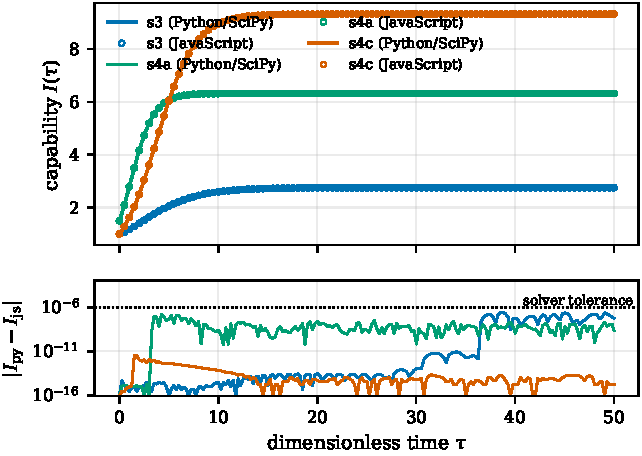
\includegraphics{figures/fig10_cross_validation.pdf}
\caption{Cross-validation of two independent implementations. Upper: capability
trajectories for three stages, Python (lines) and JavaScript (markers). Lower:
absolute difference, which stays at or below the requested solver tolerance
across the integration. The two codes share no numerical machinery.}
\label{fig:crossval}
\end{figure}

\subsection{What verification does and does not establish}

These checks establish that the equations we describe are the equations being
solved, and that they are solved accurately. They say nothing about whether the
equations describe a real civilization: no term here has been calibrated against
data, because no relevant data exist. The distinction between a verified model
and a validated one is worth keeping sharp, and we make no claim to the latter.
\Established
